% David Koch

\documentclass[
	headings=optiontotocandhead,% Erweiterung für das optionale Argument der
	% Gliederungsbefehle aktiviert.
	oneside,
	numbers=noenddot,% Keine Punkte am Ende der Gliederungsnummern und davon
	% abgeleiteten Nummern
	toc=flat, %Flache TOC --- kann man anpassen (auskommentieren)
	10pt, % Schriftgröße
	parskip=full, % Abstand zwischen Absätzen (ganze Zeile)
	listof=totoc, % Verzeichnisse im Inhaltsverzeichnis aufführen
	listof=flat, % mehr Abstand für grosse Zahlen
	numbers=noenddot, % kein Punkt am Ende bei Nummern
	%%enlargefirstpage,% Gibt es bei scrartcl nicht!!!!
	bibliography=totoc, % Literaturverzeichnis im Inhaltsverzeichnis aufführen
	%index=totoc, % Index im Inhaltsverzeichnis aufführen
	%captions=tableheading, % Beschriftung von Tabellen für Ausgabe oberhalb
	% der Tabelle formatieren
	%draft % Status des Dokuments (final/draft) draft hinzufügen zum anziegen
	%%der zeilen ende
	a4paper,DIV=14,
	% captions=tablesignature,
]{scrartcl}

\setcounter{secnumdepth}{3}

\usepackage[T1]{fontenc}
\usepackage[utf8]{inputenc}

\usepackage[english, ngerman]{babel, varioref} % your native language must be the last one!!

\usepackage{lastpage}
\usepackage{listings}
\usepackage{blindtext}

%% Aufzählungen nicht so weit einrücken
\usepackage[inline]{enumitem}
%\setitemize{leftmargin=*}
% Listen etwas wenige einrücken, erfordert enumitem
\setitemize{labelindent=2em,labelsep=0.5cm,leftmargin=12ex}

\usepackage{lmodern}

\usepackage{xspace}

\usepackage{graphicx}
\graphicspath{ {../assets} {../assets/Management} }

%%? \usepackage{textcomp}
\usepackage[hyphens]{url}
\usepackage{makeidx}
\makeindex
%%? \usepackage{graphicx}
\usepackage[numbers]{natbib}
\PassOptionsToPackage{normalem}{ulem}
\usepackage{ulem}

\usepackage{needspace}

\setlength\partopsep{0.5ex}%schoenere Listen
\usepackage[bottom]{footmisc}%fussnote ganz unten

\usepackage[]{microtype}
\UseMicrotypeSet[protrusion]{basicmath} % disable protrusion for tt fonts

\usepackage{multirow}   % Allows table elements to span several rows.
\usepackage{booktabs}   % Improves the typesettings of tables.
\usepackage{subcaption} % Allows the use of subfigures and enables their referencing.
\usepackage[ruled,linesnumbered]{algorithm2e} % Enables the writing of pseudo code.
\usepackage[usenames,dvipsnames,table]{xcolor} % Allows the definition and use of colors. This package has to be included before tikz.
\usepackage{nag}       % Issues warnings when best practices in writing LaTeX documents are violated.
\usepackage{todonotes} % Provides tooltip-like todo notes.
\usepackage{placeins}

\usepackage{color}
\usepackage[binary-units]{siunitx}

%% Override default figure placement To be within the flow of the text rather
%% than on it's own page.
% \usepackage{float}
% \makeatletter
% \def\fps@figure{H}
% \makeatother

%% bei vielen Bildern o.ä sinnvoll: Seite muss nicht bis ganz unten gefüllt werden
% \raggedbottom

%\usepackage{footbib} %  footcite, needs other tooling
%% for pandoc2 images
\makeatletter
\def\maxwidth{\ifdim\Gin@nat@width>\linewidth\linewidth\else\Gin@nat@width\fi}
\def\maxheight{\ifdim\Gin@nat@height>\textheight\textheight\else\Gin@nat@height\fi}
\makeatother
% Scale images if necessary, so that they will not overflow the page
% margins by default, and it is still possible to overwrite the defaults
% using explicit options in \includegraphics[width, height, ...]{}
\setkeys{Gin}{width=\maxwidth,height=\maxheight,keepaspectratio}

%% bessere Suche im PDF
\input{glyphtounicode}
\pdfgentounicode=1
%%%%%%%%%%%%%%%%%%%%%%%%%%%%%%%%%%%%%%%%%%%%%%%%%%%%%%%%%%%%%%%%%%%%%%%%%%%%%%%%%%

%  Kopf und Fußzeilen -- links und rechts verschieden
\newcommand{\kopfbild}{\voffset7mm
\includegraphics[width=25mm]{HTL3RLogo}}
\newcommand{\kopfHTL}{\sffamily{\textbf{\large{Projekthandbuch HTL3R}}}}

\usepackage[automark,footsepline,plainfootsepline]{scrlayer-scrpage}
\setkomafont{pageheadfoot}{\normalcolor\footnotesize\scshape}
\setkomafont{pagenumber}{\normalfont\normalsize}
\clearpairofpagestyles
\ihead{\headmark}
\ihead{\kopfbild}
\ohead{\kopfHTL}
\ifoot{\smaller{Höhere Technische Bundeslehranstalt Wien 3 | Rennweg 89b | 1030 Wien | \textcolor{orange}{www.htl.rennweg.at}}}
\ofoot{Seite \pagemark/\pageref{LastPage}}
\ModifyLayer[addvoffset=-.6ex]{scrheadings.foot.above.line}% Linie verschieben
\ModifyLayer[addvoffset=-.6ex]{plain.scrheadings.foot.above.line}% Linie verschieben
\setlength{\headheight}{32pt}

% alle Seiten mit Kopfzeile
%\renewcommand{\chapterpagestyle}{scrheadings}

%% Code Beispiele
%% eine Variante
\usepackage{listings}
\renewcommand{\lstlistingname}{\inputencoding{utf8}Listing}

\usepackage{tabularx}
\usepackage{scrhack}

\usepackage{array}
\newcommand\Tstrut{\rule{0pt}{3.2ex}}         % = `top' strut
\newcommand\Bstrut{\rule[-1.5ex]{0pt}{0pt}}   % = `bottom' strut

\newenvironment{nstabbing}
	{\setlength{\topsep}{-\parskip}
		\setlength{\partopsep}{-\parskip}
		\tabbing}
	{\endtabbing}

\usepackage{titlesec}
% \titleformat{?Überschriftenklasse?}[Absatzformatierung?]{?Textformatierung?} {?Nummerierung?}{?Abstand zwischen Nummerierung und Überschriftentext?}{?Code vor der Überschrift?}[?Code nach der Überschrift?]
\titleformat{\section}[hang]{\Large\bfseries\sffamily}{\thesection\quad}{-1.2ex}{}
\titleformat{\subsection}[hang]{\large\bfseries\sffamily}{\thesubsection\quad}{-1.2ex}{}
\titleformat{\subsubsection}[hang]{\large\bfseries\sffamily}{\thesubsubsection\quad}{-1.2ex}{}
\titleformat{\paragraph}[hang]{\large\bfseries\sffamily}{\theparagraph\quad}{-1.2ex}{}

% \titlespacing{?Überschriftenklasse?}{?Linker Einzug?}{?Platz oberhalb?}{?Platz unterhalb?}[?rechter Einzug?]
\titlespacing{\section}{0pt}{6pt}{6pt}
\titlespacing{\subsection}{0pt}{6pt}{0pt}
\titlespacing{\subsubsection}{0pt}{6pt}{0pt}
\titlespacing{\paragraph}{0pt}{6pt}{0pt}

%% sollte das letzte Package sein
\usepackage[unicode=true,
bookmarks=true,bookmarksnumbered=false,bookmarksopen=false,
breaklinks=true,pdfborder={0 0 0},backref=false,colorlinks=false]
{hyperref}
\hypersetup{pdftitle={Fenrir Management Review vom 08.10.24},
	pdfauthor={Koch, Uhlig, Burger, Vogler},
	pdfsubject={Diplomarbeit},
	pdfkeywords={5CN, DA, Fenrir}}
\urlstyle{same} % don't use monospace font for urls

% Auch Fußnoten bündig ausrichten
\deffootnote[]{1em}{1em}{\textsuperscript{\thefootnotemark\ }}
%% setup
\sloppy % weniger Meldungen
\voffset7mm % etwas nach unten

% \AddToHook{cmd/section/before}{\clearpage}

%%%%%%%%%%%%%%%%%%%%%%%%%%%%%%%%%%%%%%%%%%%%%%%%%%%%%%%%%%%%%%%%%%%%%%%%%%%%%%%%%%
\begin{document}
%% schöner: 10000 -- gar keine, 1000 als Mittelweg
\clubpenalty = 10000 % Schusterjungen verhindern
\widowpenalty = 10000 % Hurenkinder verhindern
\displaywidowpenalty = 1000

{\sffamily{\textbf{\LARGE{\textcolor{orange}{Management Review}}}}}\\
\noindent\rule{\textwidth}{0.1pt}
\begin{nstabbing}
	\hspace{4cm}\=\hspace{4cm}\=\hspace{4cm}\=\kill
	Projekttitel: \> \textbf{Fenrir}\\
	Auftraggeber: \> \textbf{Christian Schöndorfer}\\
	Auftragnehmer: \> \textbf{David Koch}\\
	Schuljahr: \> \textbf{2024/25}
	\> Klasse: \> \textbf{5CN}\\
\end{nstabbing}
{\smaller
	\begin{tabularx}{\textwidth}{l l l l}
	\hline
	\textbf{Version} & \textbf{Datum} & \textbf{Autorin/Autor} & \textbf{Änderung}\Tstrut  \\
	v1.0 & 09.10.2024 & David Koch & Erstellung des Management Reviews\Bstrut  \\
	\hline
	\end{tabularx}
}

\section{Projektstatus}
\textbf{Berichtszeitraum: 25.09.2024 bis 08.10.2024}

Derzeitiger Ampelstatus: Grün

\textbf{Termine}

{\smaller
	\begin{tabularx}{\textwidth}{|X|X|X|X|X|}
		\hline
		\textbf{\% abgeschlossen} & \textbf{Projektstatus} & \textbf{Erwartetes\newline Projektende} & \textbf{Geplantes Projektende} & \textbf{Abweichung} \\
		\hline
		26 & Grün & 14.03.2025 & 14.03.2025 & 0 \\
		\hline
	\end{tabularx}
}
% \% abgeschlossen = Prozentwert, wie viel des Gesamtprojektes abgeschlossen ist. Ermittlung auf der Basis der abgeschlossenen Arbeiten (Stunden) im Verhältnis zu den noch zu erledigenden Arbeiten (in Stunden)

\textbf{Kosten}

{\smaller
	\begin{tabularx}{\textwidth}{|X|X|X|X|X|}
		\hline
		\textbf{Ist-Kosten} & \textbf{Restkosten} & \textbf{Erwartete\newline Gesamtkosten} & \textbf{Plankosten} & \textbf{Abweichung} \\
		\hline
		- & - & - & - & - \\
		\hline
	\end{tabularx}
}
% Ist-Kosten = bisher angefallene Kosten in € / bisher angefallene Stunden \\
% Restkosten = welche Kosten bzw. wieviel Stunden sind ab heute bis zum Projektende noch zu erwarten \\
% Erwartete Gesamtkosten = Ist-Kosten + Restkosten bzw. Ist-Aufwand (h) + Restaufwand (h) \\
% Plankosten = ursprünglich (Projektbeginn, Angebot) berechnete Kosten bzw. ursprünglich geschätzter Stundenaufwand \\
% Abweichung = Erwartete Gesamtkosten – Plankosten in € bzw. Erwarteter Gesamtaufwand – Planaufwand (h) \\

\textbf{Stunden}

{\smaller
	\begin{tabularx}{\textwidth}{|X|X|X|X|X|}
		\hline
		\textbf{Ist-Aufwand} & \textbf{Restaufwand} & \textbf{Erwarteter\newline Gesamtaufwand} & \textbf{Planaufwand} & \textbf{Abweichung} \\
		\hline
		291,6 & 900,1 & 1191,7 & 1183 & +8,7 \\ % 221,6 an erledigter Arbeit + 70 in progress (zellen usw.) for good measure :)
		\hline
	\end{tabularx}
}
% Analog zu den Kosten (siehe oben)

\subsection{Teammotivation \colorbox{green!30}{:)}} 
Die Motivation ist im gesamte Team hoch, es bestehen jedoch Sorgen, dass durch zunehmenden Stress im Schuljahr die Arbeitszeit für die Diplomarbeit beeinträchtigt werden kann.

\section{Probleme im Projekt}
Es bestehen derzeit keine bemerkenswerte Probleme im Projekt. Für den ersten TOFT sollten alle OT-Betriebszellen bereits zum Teil fertig sein und da dieser bereits in ca. einem Monat ist, könnte die Arbeit an den Betriebszellen noch stressig/problematisch werden, falls bald keine Fortschritte gemacht werden.

\subsection{Problemlösungsstrategie}
So früh wie möglich (diese Woche noch) in den Baumarkt fahren und die meisten Bauteile für die dritte Betriebszelle kaufen, um diese so früh wie möglich aufzubauen und noch vor dem TOFT fertigzustellen.

\subsection{Handlungsbedarf seitens des Managements}
Notwendiger Handlungsbedarf seitens des Managements liegt in folgenden Punkten:

\begin{enumerate}
	\item Das nächste Statusmeeting mit den Betreuern ausmachen
	\item Retrospektive Zeitaufwandschätzungen für Arbeitspakete, die noch vor den Sommerferien fertiggestellt worden sind, zu tätigen
\end{enumerate}

\clearpage
\section{Erledigte Arbeiten (vollständig)}
\begin{table}[h]
	\begin{tabularx} {\textwidth} {
			|>{\hsize=.12\hsize}X
			|>{\hsize=.08\hsize}X
			|>{\hsize=.34\hsize}X
			|>{\hsize=.10\hsize}X
			|>{\hsize=.12\hsize}X
			|>{\hsize=.12\hsize}X
			|>{\hsize=.09\hsize}X|
		}
		
		\hline
		\rowcolor[HTML]{D9D9D9} 
		\textbf{\normalsize{Bearbeiter}} & \textbf{\normalsize{PSP-Code}} & {\textbf{\normalsize{Tätigkeit}}} & \textbf{\normalsize{Ort}} & \textbf{\normalsize{Dauer geplant (h)}} & \textbf{\normalsize{Dauer benötigt (h)}} & \textbf{\normalsize{Status}} \\ \hline
		Alle & 1.1.1.1 & Umfang erfassen & - & 8 & ? & \cellcolor{green!30} \\ \hline
		Alle & 1.1.1.2 & Betreuer onboarden & - & 2 & ? & \cellcolor{green!30} \\ \hline
		Alle & 1.1.1.3 & Mögliche Sponsoren/Partner erfassen & - & 4 & ? & \cellcolor{green!30} \\ \hline
		Bastian Uhlig & 1.1.2.1 & Projektidee definieren & - & 3 & 2 & \cellcolor{green!30} \\ \hline
		David Koch & 1.1.2.2 & Provisorische Projektziele definieren & - & 5 & 4,8 & \cellcolor{green!30} \\ \hline
		Gabriel Vogler & 1.1.2.3 & Stakeholder analysieren & - & 4 & 3 & \cellcolor{green!30} \\ \hline
		David Koch & 1.1.2.4 & Risikos analysieren & - & 4 & 4,5 & \cellcolor{green!30} \\ \hline
		Bastian Uhlig & 1.1.2.5 & Spielregeln definieren & - & 5 & ? & \cellcolor{green!30} \\ \hline
		Alle & 1.1.2.6 & Ansuchen schreiben & - & 10 & ? & \cellcolor{green!30} \\ \hline
		Alle & 1.1.2.7 & Antrag schreiben & - & 10 & ? & \cellcolor{green!30} \\ \hline
		David Koch & 1.2.1.1 & OSP erstellen & - & 2 & 1,8 & \cellcolor{green!30} \\ \hline
		David Koch & 1.2.1.2 & PSP erstellen & - & 3 & 3,2 & \cellcolor{green!30} \\ \hline
		Alle & 1.2.1.3 & Arbeitspakete ausdefinieren & - & 12 & ? & \cellcolor{green!30} \\ \hline
		David Koch & 1.3.1.2 & Aufbau \& Funktion der zweiten Betriebszelle planen & - & 3 & 3,9 & \cellcolor{green!30} \\ \hline
		Julian Burger & 1.3.2.3 & Provisionierung planen & - & 4 & 11 & \cellcolor{green!30} \\ \hline
		Julian Burger & 1.4.2.1 & Terraform und Packer können sich zum vSphere-Client verbinden & - & 2 & 6,5 & \cellcolor{green!30} \\ \hline
		Julian Burger & 1.4.2.2 & Packer kann eine Ubuntu-Server-VM als Template provisionieren & - & 5 & 6 & \cellcolor{green!30} \\ \hline
		Julian Burger & 1.4.2.3 & Terraform kann aus der Template von Packer eine VM aufsetzen & - & 5 & 5 & \cellcolor{green!30} \\ \hline
		Julian Burger & 1.4.2.4 & Es kann eine Bastion VM provisioniert werden & - & 15 & 15 & \cellcolor{green!30} \\ \hline
		Julian Burger & 1.4.2.5 & Über die Bastion können andere VMs leichter provisioniert werden & - & 50 & 51,5 & \cellcolor{green!30} \\ \hline
	\end{tabularx}
\end{table}
\FloatBarrier 

\begin{table}[h]
	\begin{tabularx} {\textwidth} {
			|>{\hsize=.12\hsize}X
			|>{\hsize=.08\hsize}X
			|>{\hsize=.34\hsize}X
			|>{\hsize=.10\hsize}X
			|>{\hsize=.12\hsize}X
			|>{\hsize=.12\hsize}X
			|>{\hsize=.09\hsize}X|
		}
		
		\hline
		\rowcolor[HTML]{D9D9D9} 
		\textbf{\normalsize{Bearbeiter}} & \textbf{\normalsize{PSP-Code}} & {\textbf{\normalsize{Tätigkeit}}} & \textbf{\normalsize{Ort}} & \textbf{\normalsize{Dauer geplant (h)}} & \textbf{\normalsize{Dauer benötigt (h)}} & \textbf{\normalsize{Status}} \\ \hline
		Julian Burger & 1.4.2.6 & Windows-Server Provisionierung & - & 30 & 17,5 & \cellcolor{green!30} \\ \hline
		Julian Burger & 1.4.2.7 & Windows-Client Provisionierung & - & 10 & 2,5 & \cellcolor{green!30} \\ \hline
		Julian Burger & 1.4.2.9 & Provisionierung nach gegebenem Netzplan & - & 15 & 9,25 & \cellcolor{green!30} \\ \hline
		Julian Burger & 1.5.1.1 & Webdesign festlegen & - & 5 & 5,5 & \cellcolor{green!30} \\ \hline
		David Koch & 1.5.1.2 & Randinformationen der technischen Umsetzung festlegen & - & 1 & 1,1 & \cellcolor{green!30} \\ \hline
		David Koch & 1.5.1.3 & easyname kontaktieren & - & 1,5 & 1,25 & \cellcolor{green!30} \\ \hline
		David Koch & 1.5.1.4 & Webinhalte schreiben & - & 3 & 1,4 & \cellcolor{green!30} \\ \hline
		Julian Burger & 1.5.1.5 & Website zusammenfügen & - & 8 & 6 & \cellcolor{green!30} \\ \hline
		David Koch & 1.5.2.1 & Instagram-Konto erstellen & - & 0,5 & 0,4 & \cellcolor{green!30} \\ \hline
		David Koch & 1.5.2.2 & Inhalte für Instagram desginen & - & 3 & 2,75 & \cellcolor{green!30} \\ \hline
		David Koch & 1.5.2.3 & Für das Instagram-Konto werben & - & 5 & 0,75 & \cellcolor{green!30} \\ \hline
		Bastian Uhlig & 1.5.3.1 & Fenrir-Sticker designen & - & 2 & ? & \cellcolor{green!30} \\ \hline
		Bastian Uhlig & 1.5.3.2 & Sticker bestellen & - & 1 & ? & \cellcolor{green!30} \\ \hline
		Bastian Uhlig & 1.5.3.3 & Sticker an Interessierte ausgeben & - & 1 & ? & \cellcolor{green!30} \\ \hline
	\end{tabularx}
\end{table}
\FloatBarrier 

Im Bereich der erledigten Arbeit wurden hauptsächlich Fortschritte im Bereich der Provisionierung von Windows-Servern als auch Windows-Clients gemacht. Somit konnte das gesamte IT-Netzwerk auch bereits das erste mal der Topologie nach provisioniert werden, aufgrund von Problemen mit der UCS und Schwankungen in der UCS-VPN konnte die Überprüfung dieser ersten ordentlichen Topologie-Provisionierung noch nicht vollständig durchgeführt werden.

Es wurden ebenfalls die einzelnen Netzpläne (logisch, physisch, OT) überarbeitet/erstellt und mit den ersten Adressierungskonzepten versehen.

\begin{figure}[h]
	\centering
	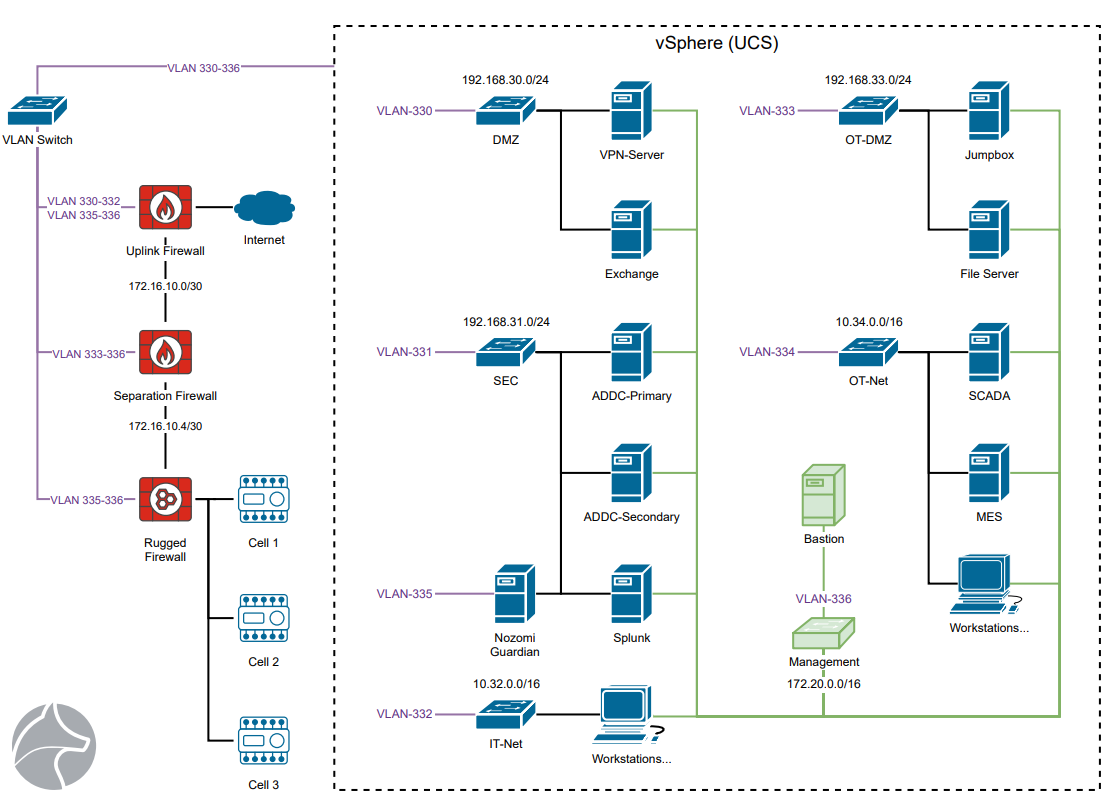
\includegraphics[width=0.9\linewidth]{20241008_1}
	\caption[]{Logischer Netzplan}
\end{figure}
\FloatBarrier 

\begin{figure}[h]
	\centering
	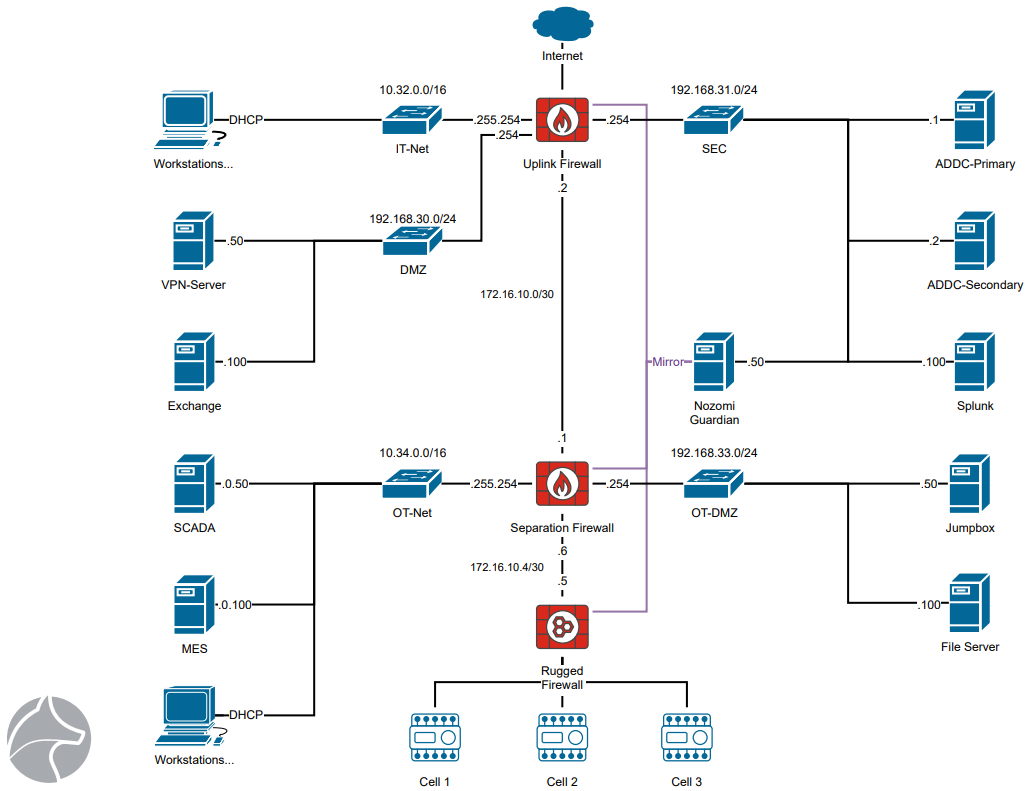
\includegraphics[width=0.9\linewidth]{20241008_2}
	\caption[]{Physischer Netzplan}
\end{figure}
\FloatBarrier 

\begin{figure}[h]
	\centering
	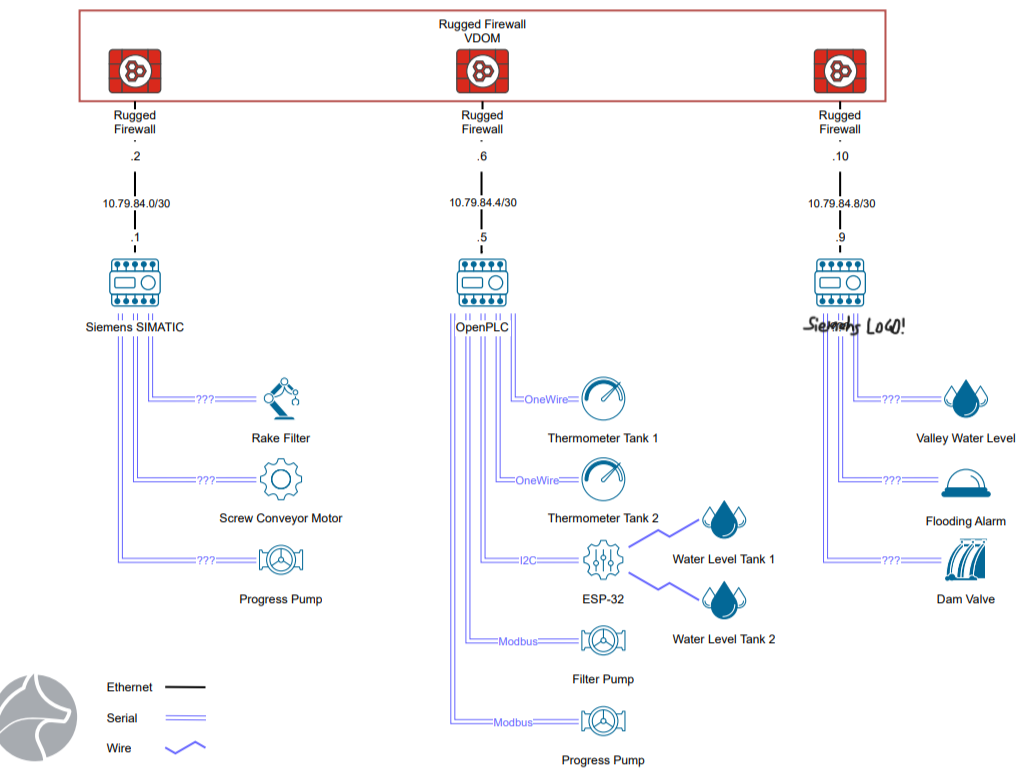
\includegraphics[width=0.9\linewidth]{20241008_3}
	\caption[]{OT-Netzplan}
\end{figure}
\FloatBarrier 

\begin{figure}[h]
	\centering
	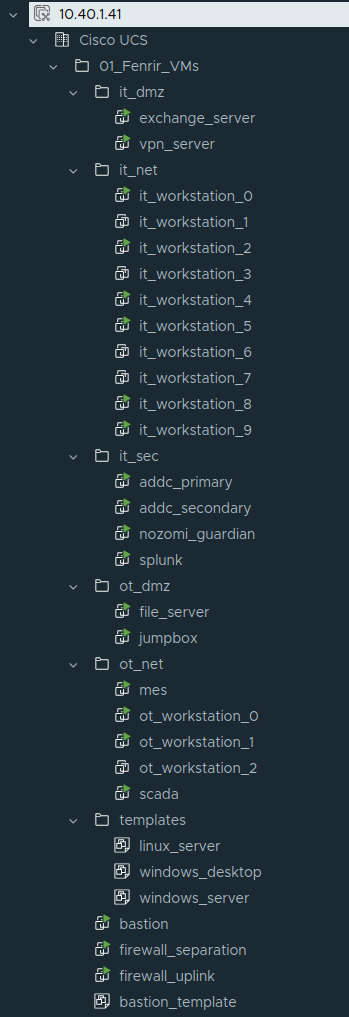
\includegraphics[width=0.9\linewidth]{20241008_4}
	\caption[]{Die provisionierten VMs im vCenter}
\end{figure}
\FloatBarrier

\clearpage
\section{Anstehende Arbeiten}
\begin{table}[h]
	\begin{tabularx} {\textwidth} {
			|>{\hsize=.12\hsize}X
			|>{\hsize=.08\hsize}X
			|>{\hsize=.54\hsize}X
			|>{\hsize=.12\hsize}X
			|>{\hsize=.15\hsize}X|
		}
		
		\hline
		\rowcolor[HTML]{D9D9D9} 
		\textbf{\normalsize{Bearbeiter}} & \textbf{\normalsize{PSP-Code}} & {\textbf{\normalsize{Tätigkeit}}} & \textbf{\normalsize{Dauer geplant (h)}} & \textbf{\smaller{Fertigstellung geplant}} \\ \hline
		David Koch & 1.3.1.1 & Aufbau \& Funktion der ersten Betriebszelle planen & 2 & 01.11.2024 \\ \hline
		Bastian Uhlig & 1.3.1.5 & SCADA-System planen & 8 & 01.11.2024 \\ \hline
		Gabriel Vogler & 1.3.2.1 & AD-Struktur planen & 6 & 20.10.2024 \\ \hline
		Gabriel Vogler & 1.3.2.2 & IT-Server planen & 4 & 08.10.2024 \\ \hline
		David Koch & 1.3.3.3 & Zellen-Firewall-Anforderungen festlegen & 3 & 20.10.2024 \\ \hline
		David Koch & 1.4.1.1 & Erste Betriebszelle aufbauen & 15 & 01.11.2024 \\ \hline
		David Koch & 1.4.1.2 & Zweite Betriebszelle aufbauen & 15 & 01.11.2024 \\ \hline
		David Koch & 1.4.1.5 & OpenPLC SPS programmieren & 5 & 05.10.2024 \\ \hline
		Julian Burger & 1.4.2.10 & Verifizierung und Überprüfung des automatischen Ablaufes & 10 & 20.10.2024 \\ \hline
		David Koch & 1.4.4.3 & Zellen-Firewall-Konfiguration(en) schreiben & 10 & 15.12.2024 \\ \hline
		Julian Burger & 1.4.4.8 & Jump Server aufgesetzt & 5 & 20.10.2024 \\ \hline
	\end{tabularx}
\end{table}

Wie zuvor erwähnt müssen aufgrund des ersten TOFT in ca. einem Monat nun alle Betriebszelle zumindest teilweise fertiggestellt werden, so, dass diese am TOFT in der Aula den Besuchern präsentiert werden können. Um die Betriebszellen auch ansteuern zu können wird ebenfalls bereits Arbeit am SCADA-System als auch an der Schnittstelle -- der Zellen-Firewall -- eingeplant.

Nach der fertigen Provisionierung von "'leeren"' Maschinen im IT-Netzwerk können diese nun auch ihre ersten Konfigurationen erhalten, wie z.B. die AD-Gerätschaft (DCs, sonstige Server, ...).

\end{document}